% \documentclass[12pt,a4paper,twoside,openright]{report}
% \let\openright=\cleardoublepage

\documentclass[12pt,a4paper]{report}


%%% Choose a language %%%

\newif\ifEN
%\ENtrue   % uncomment this for english
\ENfalse   % uncomment this for czech

%%% Configuration of the title page %%%

\def\ThesisTitleStyle{mff} % MFF style
%\def\ThesisTitleStyle{cuni} % uncomment for old-style with cuni.cz logo
%\def\ThesisTitleStyle{natur} % uncomment for nature faculty logo

\def\UKFaculty{Faculty of Mathematics and Physics}
%\def\UKFaculty{Faculty of Science}

\def\UKName{Charles University in Prague} % this is not used in the "mff" style

% Thesis type names, as used in several places in the title
\def\ThesisTypeTitle{\ifEN BACHELOR THESIS \else BAKALÁŘSKÁ PRÁCE \fi}
%\def\ThesisTypeTitle{\ifEN MASTER THESIS \else DIPLOMOVÁ PRÁCE \fi}
%\def\ThesisTypeTitle{\ifEN RIGOROUS THESIS \else RIGORÓZNÍ PRÁCE \fi}
%\def\ThesisTypeTitle{\ifEN DOCTORAL THESIS \else DISERTAČNÍ PRÁCE \fi}
\def\ThesisGenitive{\ifEN bachelor \else bakalářské \fi}
%\def\ThesisGenitive{\ifEN master \else diplomové \fi}
%\def\ThesisGenitive{\ifEN rigorous \else rigorózní \fi}
%\def\ThesisGenitive{\ifEN doctoral \else disertační \fi}
\def\ThesisAccusative{\ifEN bachelor \else bakalářskou \fi}
%\def\ThesisAccusative{\ifEN master \else diplomovou \fi}
%\def\ThesisAccusative{\ifEN rigorous \else rigorózní \fi}
%\def\ThesisAccusative{\ifEN doctoral \else disertační \fi}



%%% Fill in your details %%%

% (Note: \xxx is a "ToDo label" which makes the unfilled visible. Remove it.)
\def\ThesisTitle{Detekcia anonymizovaných častí v~zmluvách}
\def\ThesisAuthor{Lukáš Salak}
\def\YearSubmitted{2024}

% department assigned to the thesis
\def\Department{Katedra softwaru a výuky informatiky}
% Is it a department (katedra), or an institute (ústav)?
\def\DeptType{Katedra}

\def\Supervisor{doc. RNDr. Elena Šikudová, Ph.D.}
\def\SupervisorsDepartment{Katedra softwaru a~výuky informatiky}

% Study programme and specialization
\def\StudyProgramme{Informatika}
\def\StudyBranch{Počítačová grafika, vidění a vývoj her}

\def\Dedication{%
Dedikácia. Nesmierne si cením podpory a pomoci, ktorú som dostal od mnohých ľudí, 
menovite od mojej rodiny, mojej priateľky, priateľov, spolužiakov a kolegov. Najviac však by som chcel 
poďakovať vedúcej mojej bakalárskej práce,
doc. RNDr. Elene Šikudovej, Ph.D., ktorá mi pomohla pri všetkom, čo som potreboval.
}

\def\AbstractEN{%
The work examines the problem of detecting anonymized parts in PDF documents. Various detection approaches, primarily image analysis and related computer vision algorithms, were explored. We implemented and evaluated the best of these approaches on test data. The results showed that the implemented approach achieved high accuracy and outperformed other approaches also in terms of efficiency. This research contributes to the development of tools to help analyze documents that can be applied in various legal or financial areas to guarantee data protection in accordance with regulations.
}

\def\ProposalEN{%
The goal is to calculate the ratio of anonymized parts in given PDF - that cna be either blackened, overlayed with noise or whitened completely. The work will consist of an introduction to the issue and analysis of the problem, proposals for the procedures, selection and implementation of analytical operations over PDF, comparison of individual approaches to the problem and outputs of individual operations and the resulting statistics, which will be the output of the implemented program.
}

\def\AbstractSK{%
\begin{hyphenrules}{nohyphenation}
Práca skúma problém detegovania anonymizovaných častí v PDF dokumentoch. Preskúmané  boli rôzne prístupy na detekciu, primárne analýza obrazu a s ňou spojené rôzne algoritmy počítačového videnia. Najlepší z týchto prístupov sme implementovali a vyhodnotili na testovacích dátach. Výsledky ukázali, že implementovaný prístup dosiahol vysokú presnosť a predbehol iné prístupy aj vzhľadom na efektivitu. Tento výskum prispieva k rozvoju nástrojov pomáhajúcich analyzovať dokumenty, ktoré môžu byť aplikované v~rôznych právnych či finančných oblastiach na zaručenie ochrany dát v~súlade s~reguláciami.
\end{hyphenrules}
}

\def\ProposalSK{%
Cieľom je v zadanom PDF spočítať začiernenú plochu - môže byť buď začiernená, zaplnená zrnením či prípadne zabielená. Obsahom práce bude uvedenie do problematiky a analýza problému, návrhy postupu, výber a implementácia analytických operácií nad PDF, porovnanie jednotlivých prístupov k problému a výstupy jednotlivých opercií a výsledná štatistika, ktorá bude výstupom implementovaného programu.
}



% 3 to 5 keywords (recommended), each enclosed in curly braces.
% Keywords are useful for indexing and searching for the theses by topic.
\def\Keywords{%
{PDF, Segmentace, Detekce}
}

% If your abstracts are long and do not fit in the infopage, you can make the
% fonts a bit smaller by this setting. (Also, you should try to compress your abstract more.)
% Alternatively, consider increasing the size of the page by uncommenting the
% geometry modification in thesis.tex.
\def\InfoPageFont{}
%\def\InfoPageFont{\small}  %uncomment to decrease font size

\ifEN\relax\else
% If you are writing a czech thesis, you additionally need to fill in the
% english translation of the metadata here!
\def\ThesisTitleEN{Detection of anonymized parts in PDFs}
\def\DepartmentEN{Department of Software and Computer Science Education}
\def\DeptTypeEN{Department}
\def\SupervisorsDepartmentEN{Department of Software \newline and~Computer Science Education}
\def\StudyProgrammeEN{Computer Science}
\def\StudyBranchEN{Computer Graphics, Vision and Game Development}
\def\KeywordsEN{%
{PDF, Segmentation, Detection}
}
\fi

\newenvironment{specialpar}[1]{\par#1}{\par}

\usepackage[a-2u]{pdfx}

\ifEN\else\usepackage[czech,shorthands=off]{babel}\fi
\usepackage[utf8]{inputenc}
\usepackage[T1]{fontenc}

% See https://en.wikipedia.org/wiki/Canons_of_page_construction before
% modifying the size of printable area. LaTeX defaults are great.
% If you feel it would help anything, you can enlarge the printable area a bit:
%\usepackage[textwidth=390pt,textheight=630pt]{geometry}
% The official recommendation expands the area quite a bit (looks pretty harsh):
%\usepackage[textwidth=145mm,textheight=247mm]{geometry}

%%% FONTS %%%
\usepackage{lmodern} % TeX "original" (this sets up the latin mono)

% Optionally choose an override for the main font for typesetting:
\usepackage[mono=false]{libertinus} % popular for comp-sci (ACM uses this)
%\usepackage{tgschola} % Schoolbook-like (gives a bit of historic feel)
%\usepackage[scale=0.96]{tgpagella} % Palladio-like (popular in formal logic).
% IBM Plex font suite is nice but requires us to fine-tune the sizes, also note
% that it does not directly support small caps (\textsc) and requires lualatex:
%\usepackage[usefilenames,RM={Scale=0.88},SS={Scale=0.88},SScon={Scale=0.88},TT={Scale=0.88},DefaultFeatures={Ligatures=Common}]{plex-otf}

% Optionally choose a custom sans-serif fonts (e.g. for figures and tables).
% Default sans-serif font is usually Latin Modern Sans. Some font packages
% (e.g. libertinus) replace that with a better matching sans-serif font.
%\usepackage{tgheros} % recommended and very readable (Helvetica-like)
%\usepackage{FiraSans} % looks great
% DO NOT typeset the main text in sans-serif font!
% The serifs make the text easily readable on the paper.

% IMPORTANT FONT NOTE: Some fonts require additional PDF/A conversion using
% the pdfa.sh script. These currently include only 'tgpagella'; but various
% other fonts from the texlive distribution need that too (mainly the Droid
% font family).


% some useful packages
\usepackage{microtype}
\usepackage{amsmath,amsfonts,amsthm,bm}
\usepackage{graphicx}
\usepackage{xcolor}
\usepackage{booktabs}
\usepackage{caption}
\usepackage{floatrow}

% load bibliography tools
\usepackage[backend=bibtex,natbib,style=numeric,sorting=none]{biblatex}
% alternative with alphanumeric citations (more informative than numbers):
%\usepackage[backend=bibtex,natbib,style=alphabetic]{biblatex}
%
% alternatives that conform to iso690
% (iso690 is not formally required on MFF, but may help elsewhere):
%\usepackage[backend=bibtex,natbib,style=iso-numeric,sorting=none]{biblatex}
%\usepackage[backend=bibtex,natbib,style=iso-alphabetic]{biblatex}
%
% additional option choices:
%  - add `giveninits=true` to typeset "E. A. Poe" instead of full Edgar Allan
%  - `terseinits=true` additionaly shortens it to nature-like "Poe EA"
%  - add `maxnames=10` to limit (or loosen) the maximum number of authors in
%    bibliography entry before shortening to `et al.` (useful when referring to
%    book collections that may have hundreds of authors)
%  - for additional flexibility (e.g. multiple reference sections, etc.),
%    remove `backend=bibtex` and compile with `biber` instead of `bibtex` (see
%    Makefile)
%  - `sorting=none` causes the bibliography list to be ordered by the order of
%    citation as they appear in the text, which is usually the desired behavior
%    with numeric citations. Additionally you can use a style like
%    `numeric-comp` that compresses the long lists of citations such as
%    [1,2,3,4,5,6,7,8] to simpler [1--8]. This is especially useful if you plan
%    to add tremendous amounts of citations, as usual in life sciences and
%    bioinformatics.
%  - if you don't like the "In:" appearing in the bibliography, use the
%    extended style (`ext-numeric` or `ext-alphabetic`), and add option
%    `articlein=false`.
%
% possibly reverse the names of the authors with the default styles:
%\DeclareNameAlias{default}{family-given}

% load the file with bibliography entries
\addbibresource{refs}

% remove this if you won't use fancy verbatim environments
\usepackage{fancyvrb}

% remove this if you won't typeset TikZ graphics
\usepackage{tikz}
\usetikzlibrary{positioning} %add libraries as needed (shapes, decorations, ...)

% remove this if you won't typeset any pseudocode
\usepackage{algpseudocode}
\usepackage{algorithm}

% remove this if you won't list any source code
\usepackage{listings}


\hypersetup{unicode}
\hypersetup{breaklinks=true}

\usepackage[noabbrev]{cleveref}


% various forms of TODOs (you should remove this before submitting)
\usepackage[textsize=tiny, backgroundcolor=yellow!25, linecolor=black!25]{todonotes}
\newcommand{\xxx}[1]{\textcolor{red!}{#1}}

 % remove this before compiling the final version


% use this for typesetting a chapter without a number, e.g. intro and outro
\def\chapwithtoc#1{
\chapter*{#1}
\addcontentsline{toc}{chapter}{#1}
}

% If there is a line/figure overflowing into page margin, this will make the
% problem evident by drawing a thick black line at the overflowing spot. You
% should not disable this.
\overfullrule=3mm

% The maximum stretching of a space. Increasing this makes the text a bit more
% sloppy, but may prevent the overflows by moving words to next line.
\emergencystretch=1em

\ifEN
\theoremstyle{plain}
\newtheorem{thm}{Theorem}
\newtheorem{lemma}[thm]{Lemma}
\newtheorem{claim}[thm]{Claim}
\newtheorem{defn}{Definition}
\theoremstyle{remark}
\newtheorem*{cor}{Corollary}
\else
\theoremstyle{plain}
\newtheorem{thm}{Veta}
\newtheorem{lemma}{Lemma}
\newtheorem{claim}{Tvrdenie}
\newtheorem{defn}{Definícia}
\theoremstyle{remark}
\newtheorem*{cor}{Dôsledok}
\fi

\newenvironment{myproof}{
  \par\medskip\noindent
  \textit{\ifEN Proof \else Dôkaz \fi}.
}{
\newline
\rightline{$\qedsymbol$}
}

% real/natural numbers
\newcommand{\R}{\mathbb{R}}
\newcommand{\N}{\mathbb{N}}

% asymptotic complexity
\newcommand{\asy}[1]{\mathcal{O}(#1)}

% listings and default lstlisting config (remove if unused)
\DeclareNewFloatType{listing}{}
\floatsetup[listing]{style=ruled}

\DeclareCaptionStyle{thesis}{style=base,font={small,sf},labelfont=bf,labelsep=quad}
\captionsetup{style=thesis}
\captionsetup[algorithm]{style=thesis,singlelinecheck=off}
\captionsetup[listing]{style=thesis,singlelinecheck=off}

% Customization of algorithmic environment (comment style)
\renewcommand{\algorithmiccomment}[1]{\textcolor{black!25}{\dotfill\sffamily\itshape#1}}

% Uncomment for table captions on top. This is sometimes recommended by the
% style guide, and even required for some publication types.
%\floatsetup[table]{capposition=top}
%
% (Opinionated rant:) Captions on top are not "compatible" with the general
% guideline that the tables should be formatted to be quickly visually
% comprehensible and *beautiful* in general (like figures), and that the table
% "head" row (with column names) should alone communicate most of the content
% and interpretation of the table. If you just need to show a long boring list
% of numbers (because you have to), either put some effort into showing the
% data in an attractive figure-table, or move the data to an attachment and
% refer to it, so that the boredom does not impact the main text flow.
%
% You can make the top-captions look much less ugly by aligning the widths of
% the caption and the table, with setting `framefit=yes`, as shown below.  This
% additionally requires some extra markup in your {table} environments; see the
% comments in the example table in `ch2.tex` for details.
%\floatsetup[table]{capposition=top,framefit=yes}

\ifEN\floatname{listing}{Listing}
\else\floatname{listing}{Výpis kódu}\fi
\lstset{ % use this to define styling for any other language
  language=C++,
  tabsize=2,
  showstringspaces=false,
  basicstyle=\footnotesize\tt\color{black!75},
  identifierstyle=\bfseries\color{black},
  commentstyle=\color{green!50!black},
  stringstyle=\color{red!50!black},
  keywordstyle=\color{blue!75!black}}

% Czech versions of the used cleveref references (It's not as convenient as in
% English because of declension, cleveref is limited to sg/pl nominative. Use
% plain \ref to dodge that.)
\ifEN\relax\else
\crefname{chapter}{kapitola}{kapitoly}
\Crefname{chapter}{Kapitola}{Kapitoly}
\crefname{section}{sekcia}{sekcie}
\Crefname{section}{Sekcia}{Sekcie}
\crefname{subsection}{sekcia}{sekcie}
\Crefname{subsection}{Sekcia}{Sekcie}
\crefname{subsubsection}{sekcia}{sekcie}
\Crefname{subsubsection}{Sekcia}{Sekcie}
\crefname{figure}{obrázok}{obrázky}
\Crefname{figure}{Obrázok}{Obrázky}
\crefname{table}{tabuľka}{tabuľky}
\Crefname{table}{Tabuľka}{Tabuľky}
\crefname{listing}{výpis}{výpisy}
\Crefname{listing}{Výpis}{Výpisy}
\floatname{algorithm}{Algoritmus}
\crefname{algorithm}{algoritmus}{algoritmy}
\Crefname{algorithm}{Algoritmus}{Algoritmy}
\newcommand{\crefpairconjunction}{ a~}
\newcommand{\crefrangeconjunction}{ a~}
\fi
 % use this file for various custom definitions


\begin{document}

% the layout is mandatory, edit only in dire circumstances

\pagestyle{empty}
\hypersetup{pageanchor=false}
\begin{center}

% top part of the layout, this actually differs between faculties

\def\ThesisTitleXmff{%
  \ifEN
    \centerline{\mbox{
\includegraphics[width=166mm]{img/logo-en.pdf}}}
  \else
    \centerline{\mbox{
\includegraphics[width=166mm]{img/logo-cs.pdf}}}
  \fi
  \vspace{-8mm}\vfill%
  {\bf\Large\ThesisTypeTitle}
  \vfill%
  {\LARGE\ThesisAuthor}\par
  \vspace{15mm}%
  {\LARGE\bfseries\ThesisTitle}
  \vfill%
  \Department}
\def\ThesisTitleCuniLogo#1{%
  {\large\UKName\par\medskip\par\UKFaculty }
  \vfill%
  {\bf\Large\ThesisTypeTitle}
  \vfill%
  \includegraphics[width=70mm]{#1}
  \vfill%
  {\LARGE\ThesisAuthor}\par
  \vspace{15mm}%
  {\LARGE\bfseries\ThesisTitle}
  \vfill%
  \Department\par}
\def\ThesisTitleXcuni{\ThesisTitleCuniLogo{img/uklogo.pdf}}
\def\ThesisTitleXnatur{\ThesisTitleCuniLogo{img/naturlogo.pdf}}

% choose the correct page and print it
\csname ThesisTitleX\ThesisTitleStyle\endcsname
% latex corner: X is the new @

\vfill

{
\centerline{\vbox{\halign{\hbox to 0.45\hsize{\hfil #}&\hskip 0.5em\parbox[t]{0.45\hsize}{\raggedright #}\cr
\ifEN Supervisor of the \ThesisGenitive thesis:
\else Vedúci \ThesisGenitive práce: \fi
& \Supervisor \cr
\noalign{\vspace{2mm}}
\ifEN Study programme: \else Študijný program: \fi
& \StudyProgramme \cr
\noalign{\vspace{2mm}}
\ifEN Study branch: \else Študijný obor: \fi
& \StudyBranch \cr
}}}}

\vfill

\ifEN Prague \else Praha \fi
\YearSubmitted

\end{center}

\newpage

% remember to sign this!
%\openright
\hypersetup{pageanchor=true}
\pagestyle{plain}
\pagenumbering{roman}
\vglue 0pt plus 1fill

\ifEN
\noindent
I declare that I carried out this \ThesisAccusative thesis independently, and only with the cited
sources, literature and other professional sources. It has not been used to obtain another
or the same degree.
\else
\noindent
Prohlašuji, že jsem tuto \ThesisAccusative práci vypracoval(a) samostatně a výhradně
s~použitím citovaných pramenů, literatury a dalších odborných zdrojů.
Tato práce nebyla využita k získání jiného nebo stejného titulu.
\fi

\ifEN
\medskip\noindent
I understand that my work relates to the rights and obligations under the Act No.~121/2000 Sb.,
the Copyright Act, as amended, in particular the fact that the Charles
University has the right to conclude a license agreement on the use of this
work as a school work pursuant to Section 60 subsection 1 of the Copyright~Act.
\else
\medskip\noindent
Beru na~vědomí, že se na moji práci vztahují práva a povinnosti vyplývající
ze zákona č. 121/2000 Sb., autorského zákona v~platném znění, zejména skutečnost,
že Univerzita Karlova má právo na~uzavření licenční smlouvy o~užití této
práce jako školního díla podle §60 odst. 1 autorského zákona.
\fi

\vspace{10mm}


\ifEN
\hbox{\hbox to 0.5\hsize{%
In \hbox to 6em{\dotfill} date \hbox to 6em{\dotfill}
\hss}\hbox to 0.5\hsize{\dotfill\quad}}
\smallskip
\hbox{\hbox to 0.5\hsize{}\hbox to 0.5\hsize{\hfil Author's signature\hfil}}
\else
\hbox{\hbox to 0.5\hsize{%
V \hbox to 6em{\dotfill} dne \hbox to 6em{\dotfill}
\hss}\hbox to 0.5\hsize{\dotfill\quad}}
\smallskip
\hbox{\hbox to 0.5\hsize{}\hbox to 0.5\hsize{\hfil Podpis autora\hfil}}
\fi

\vspace{20mm}
\newpage

% dedication

%\openright

\noindent
\Dedication

\newpage

% mandatory information page

%\openright

\vbox to 0.49\vsize{\InfoPageFont
\setlength\parindent{0mm}
\setlength\parskip{5mm}

\ifEN Title: \else Názov práce: \fi
\ThesisTitle

\ifEN Author: \else Autor: \fi
\ThesisAuthor

\DeptType:
\Department

\ifEN Supervisor: \else Vedúci \ThesisGenitive práce: \fi
\Supervisor, \SupervisorsDepartment

\ifEN Abstract: \AbstractEN \else Abstrakt: \AbstractCS \fi

\ifEN Keywords: \else Kľúčové slová: \fi
\Keywords

\vss}\ifEN\relax\else\nobreak\vbox to 0.49\vsize{\InfoPageFont
\setlength\parindent{0mm}
\setlength\parskip{5mm}

Title:
\ThesisTitleEN

Author:
\ThesisAuthor

\DeptTypeEN:
\DepartmentEN

Supervisor:
\Supervisor, \SupervisorsDepartmentEN

Abstract:
\AbstractEN

Keywords:
\KeywordsEN

\vss}
\fi

\newpage

%\openright
\pagestyle{plain}
\pagenumbering{arabic}
\setcounter{page}{1}


\tableofcontents
\chapwithtoc{Úvod}
\label{chap:intro}
%\todo[inline]{Sem by som asi nedavala ziadne section}
Problém anonymizácie dát je dôležitý v rôznych oblastiach, napríklad v oblasti verejnej správy či
v oblasti marketingu. Pod pojmom anonymizácia dokumentov si môžeme predstaviť vymazanie či skrytie údajov 
alebo iných citlivých informácií. Možností, ako pristupovať k anonymizácii dokumentov, je veľa. 
\newline

Typickým miestom, kde sa stretávame s anonymizáciou dokumentov, je oblasť verejnej správy.
V Českej republike majú organizácie verejnej správy povinnosť zverejňovať informácie o svojej činnosti,
k čomu patrí aj zverejňovanie uzavretých zmlúv nad určitú čiastku do \textit{registra zmlúv}, 
ktorý je verejne prístupný. Nachádzajú sa tu nielen informácie o predmete zmlúv, zmluvných stranách a cene,
ale takisto všetky súbory, ktoré sú súčasťou zmlúv. Register zmlúv je významným nástrojom, ktorý zlepšuje 
transparentnosť; podstatou je kontrolovať a mať možnosť obmedziť korupciu a zneužívanie verejnej moci 
kvôli uzatváraniu nevýhodných zmlúv.
\newline

Aj napriek tomu, že zverejňovanie dát v registri zmlúv je právne vynútiteľné, nezabezpečuje to automaticky
možnosť jednoduchého vyhľadávania či analýzy týchto dát. K tomu bol vytvorený projekt, webový portál 
\textit{Hlídač smluv}, ktorý má za úlohu zlepšiť prístup k registru zmlúv. Neskôr, po skombinovaní ďalších 
verejne prístupných dát z registrov a databáz, sa vytvoril projekt Hlídač státu \cite{HlidacStatu}, ktorý má za úlohu zlepšiť prístup k verejným informáciám. Poskytuje
napríklad plnohodnotné vyhľadávanie v texte zmlúv.
\newline


\begin{hyphenrules}{nohyphenation}
V registri zmlúv sú dokumenty z rôznych oblastí, napríklad z oblasti zdravotníctva, školstva, realitných služieb alebo
IT projektov. V prípade, že dokumenty obsahujú citlivé údaje, sú častokrát anonymizované. V súčasnej dobe neexistuje 
štatistický nástroj, ktorý by znázorňoval koľko percent v takýchto dokumentoch je zanonymizovaných.
\end{hyphenrules}

\newpage

\begin{hyphenrules}{nohyphenation}
Cieľom práce je zaoberať sa anonymizovanými PDF dokumentmi a vytvorenie nástroja, 
ktorý bude schopný detegovať anonymizované časti dokumentu, využiť grafické metódy používané pri počítačovom videní a ďalších algoritmov na spracovanie obrazu a navrhnúť tak systém, ktorý umožní na základe dostupných dát vyhodnotiť percento anonymizácie jednotlivých zmlúv pri použití konkrétnych implementačných metód a následne nasadiť túto implementáciu na webový portál Hlídače státu.
\newline

Hlavným prínosom práce je vytvorenie systému na porovnávanie jednotlivých odvetví, ktoré zverejňujú zmluvy vzhľadom na percento anonymizácie a
tvorba štatistiky vzhľadom na anonymizáciu dokumentov relatívne k jednotlivým oblastiam.
\newline

Práca je štruktúrovaná nasledovne: \ref{chap:FirstChapter}. kapitola rieši definíciu anonymizácie, právne aspekty a dôvody pre anonymizáciu a možné metódy a techniky, ktorými sa dokumenty anonymizujú. V \ref{chap:SecondChapter}. kapitole je špecifikovaný konkrétny problém a~zadanie, ktorému sa v práci venujeme. \ref{chap:ThirdChapter}. kapitola je venovaná popisu vstupných dát, ich obsah a štruktúra. Takisto je tu popísaný proces získavania dát a ich príprava na ďalšie spracovanie a extrakcia relevantných informácií. V \ref{chap:FourthChapter}. kapitole je popísaný proces detekcie anonymizovaných častí dokumentov. V kapitole \ref{chap:FifthChapter} je popísaný algoritmus, ktorý v systéme používame.
\Cref{chap:SixthChapter} je venovaná implementácii riešenia, použité technológie a nástroje, architektúra a dizajn systému, prípadové štúdie a ďalšie detaily implementácie. V závere kapitoly \ref{chap:conclusion} zhŕňame mimo dosiahnutých výsledkov aj osobné zistenia a odporúčania pre ďalší výskum.  
\end{hyphenrules}
\chapter{Register zmlúv, zverejňovanie a anonymizácia dokumentov}
\label{chap:FirstChapter}

% First chapter usually builds the theoretical background necessary for readers to understand the rest of the thesis. You should summarize and reference a lot of existing literature and research.

% You should use the standard \emph{citations}\todo{Use \textbackslash{}emph command like this, to highlight the first occurrence of an important word or term. Reader will notice it, and hopefully remember the importance.}.

% \begin{description}
% \item[Obtaining bibTeX citation] Go to Google Scholar\footnote{\url{https://scholar.google.com}}\todo{This footnote is an acceptable way to `cite' webpages or URLs. Documents without proper titles, authors and publishers generally do not form citations. For this reason, avoid citations of wikipedia pages.}, find the relevant literature, click the tiny double-quote button below the link, and copy the bibTeX entry.
% \item[Saving the citation] Insert the bibTeX entry to the file \texttt{refs.bib}. On the first line of the entry you should see the short reference name --- from Scholar, it usually looks like \texttt{author2015title} --- you will use that to refer to the citation.
% \item[Using the citation] Use the \verb|\cite| command to typeset the citation number correctly in the text; a long citation description will be automaticaly added to the bibliography at the end of the thesis. Always use a non-breakable space before the citing parenthesis to avoid unacceptable line breaks:
% \begin{Verbatim}
% Trees utilize gravity to invade ye
% noble sires~\cite{newton1666apple}.
% \end{Verbatim}
% \item[Why should I bother with citations at all?] For two main reasons:
% \begin{itemize}
% \item You do not have to explain everything in the thesis; instead you send the reader to refer to details in some other literature. Use citations to simplify the detailed explanations.
% \item If you describe something that already exists without using a citation, the reviewer may think that you \emph{claim} to have invented it. Expectably, they will demand academic correctness, and, from your perspective, being accused of plagiarism is not a good starting point for a successful defense. Use citations to identify the people who invented the ideas that you build upon.
% \end{itemize}
% \item[How many citations should I use?]
% Cite any non-trivial building block or assumption that you use, if it is published in the literature. You do not have to cite trivia, such as the basic definitions taught in the introductory courses.

% The rule of thumb is that you should read, understand and briefly review at least around 4 scientific papers. A thesis that contains less than 3 sound citations will spark doubt in reviewers.
% \end{description}

% There are several main commands for inserting citations, used as follows:
% \begin{itemize}
% \item \citet{knuth1979tex} described a great system for typesetting theses.
% \item We are typesetting this thesis with \LaTeX, which is based on \TeX{} and METAFONT~\cite{knuth1979tex}.
% \item \TeX{} was expanded to \LaTeX{} by \citet{lamport1994latex}, hence the name.
% \item Revered are the authors of these systems!~\cite{knuth1979tex,lamport1994latex}
% \end{itemize}

% \section{Some extra assorted hints before you start writing English}

% Strictly adhere to the English word order rules. The sentences follow a fixed structure with a subject followed by a verb and an object (in this order). Exceptions to this rule must be handled specially, and usually separated by commas.

% Mind the rules for placing commas:
% \begin{itemize}
% \item Use the \emph{Oxford comma} before `and' and `or' at the end of a longer, comma-separated list of items. Certainly use it to disambiguate any possible mixtures of conjunctions: \textit{`The car is available in red, red and green, and green versions.'}
% \item Do not use the comma before subordinate clauses that begin with `that' (like this one). English does not use subordinate clauses as often as Slavic languages because the lack of a suitable word inflection method makes them hard to understand. In scientific English, try to avoid them as much as possible. Ask doubtfully whether each `which' and `when' is necessary --- most of these helper conjunctions can be removed by converting the clause to non-subordinate.

% As an usual example, \xxx{\textit{`The sentence, which I wrote, seemed ugly.'}} is perfectly bad; slightly improved by \xxx{\textit{`The sentence that I wrote seemed ugly.'}}, which can be easily reduced to \textit{`The sentence I wrote seemed ugly.'}. A final version with added storytelling value could say \textit{`I wrote a sentence but it seemed ugly.'}
% \item Consider placing extra commas around any parts of the sentence that break the usual word order, especially if they are longer than a single word.
% \end{itemize}

% Do not write long sentences. One sentence should contain exactly one fact. Multiple facts should be grouped in a paragraph to communicate one coherent idea. Paragraphs are grouped in labeled sections for a sole purpose of making the navigation in the thesis easier. Do not use the headings as `names for paragraphs' --- the text should make perfect sense even if all headings are removed. If a section of your text contains one paragraph per heading, you might have wanted to write an explicit list instead.

% Every noun needs a determiner (`a', `the', `my', `some', \dots); the exceptions to this rule, such as non-adjectivized names and indeterminate plural, are relatively scarce. Without a determiner, a noun can be easily mistaken for something completely different, such as an adjective or a verb.

% Consult the books by \citet{glasman2010science} and \citet{sparling1989english} for more useful details.

\chapter{Špecifikácia problému}
\label{chap:SecondChapter}

% After the reader gained sufficient knowledge to understand your problem in \cref{chap:refs}, you can jump to your own advanced material and conclusions.

% You will need definitions (see \cref{defn:x} below in \cref{sec:demo}), theorems (\cref{thm:y}), general mathematics, algorithms (\cref{alg:w}), and tables (\cref{tab:z})\todo{See documentation of package \texttt{booktabs} for hints on typesetting tables. As a main rule, \emph{never} draw a vertical line.}. \Cref{fig:f,fig:g} show how to make a nice figure. See \cref{fig:schema} for an example of TikZ-based diagram. Cross-referencing helps a lot to keep the necessary parts of the narrative close --- use references to the previous chapter with theory wherever it seems that the reader could have forgotten the required context.

% \section{Example with some mathematics}
% \label{sec:demo}

% \begin{defn}[Triplet]\label{defn:x}
% Given stuff $X$, $Y$ and $Z$, we will write a \emph{triplet} of the stuff as $(X,Y,Z)$.
% \end{defn}

% \newcommand{\Col}{\textsc{Colour}}

% \begin{thm}[Car coloring]\label{thm:y}
% All cars have the same color. More specifically, for any set of cars $C$, we have
% $$(\forall c_1, c_2 \in C)\:\Col(c_1) = \Col(c_2).$$
% \end{thm}

% \begin{proof}
% Use induction on sets of cars $C$. The statement holds trivially for $|C|\leq1$. For larger $C$, select 2 overlapping subsets of $C$ smaller than $|C|$ (thus same-colored). Overlapping cars need to have the same color as the cars outside the overlap, thus also the whole $C$ is same-colored.\todo{This is plain wrong though.}
% \end{proof}

% \begin{table}
% % uncomment the following line if you use the fitted top captions for tables
% % (see the \floatsetup[table] comments in `macros.tex`.
% %\floatbox{table}[\FBwidth]{
% \centering\footnotesize\sf
% \begin{tabular}{llrl}
% \toprule
% Column A & Column 2 & Numbers & More \\
% \midrule
% Asd & QWERTY & 123123 & -- \\
% Asd qsd 1sd & \textcolor{red}{BAD} & 234234234 & This line should be helpful. \\
% Asd & \textcolor{blue}{INTERESTING} & 123123123 & -- \\
% Asd qsd 1sd & \textcolor{violet!50}{PLAIN WEIRD} & 234234234 & -- \\
% Asd & QWERTY & 123123 & -- \\
% \addlinespace % a nice non-intrusive separator of data groups (or final table sums)
% Asd qsd 1sd & \textcolor{green!80!black}{GOOD} & 234234299 & -- \\
% Asd & NUMBER & \textbf{123123} & -- \\
% Asd qsd 1sd & DIFFERENT & 234234234 & (no data) \\
% \bottomrule
% \end{tabular}
% %}{  % uncomment if you use the \floatbox (as above), erase otherwise
% \caption{An example table.  Table caption should clearly explain how to interpret the data in the table. Use some visual guide, such as boldface or color coding, to highlight the most important results (e.g., comparison winners).}
% %}  % uncomment if you use the \floatbox
% \label{tab:z}
% \end{table}

% \begin{figure}
% \centering
% 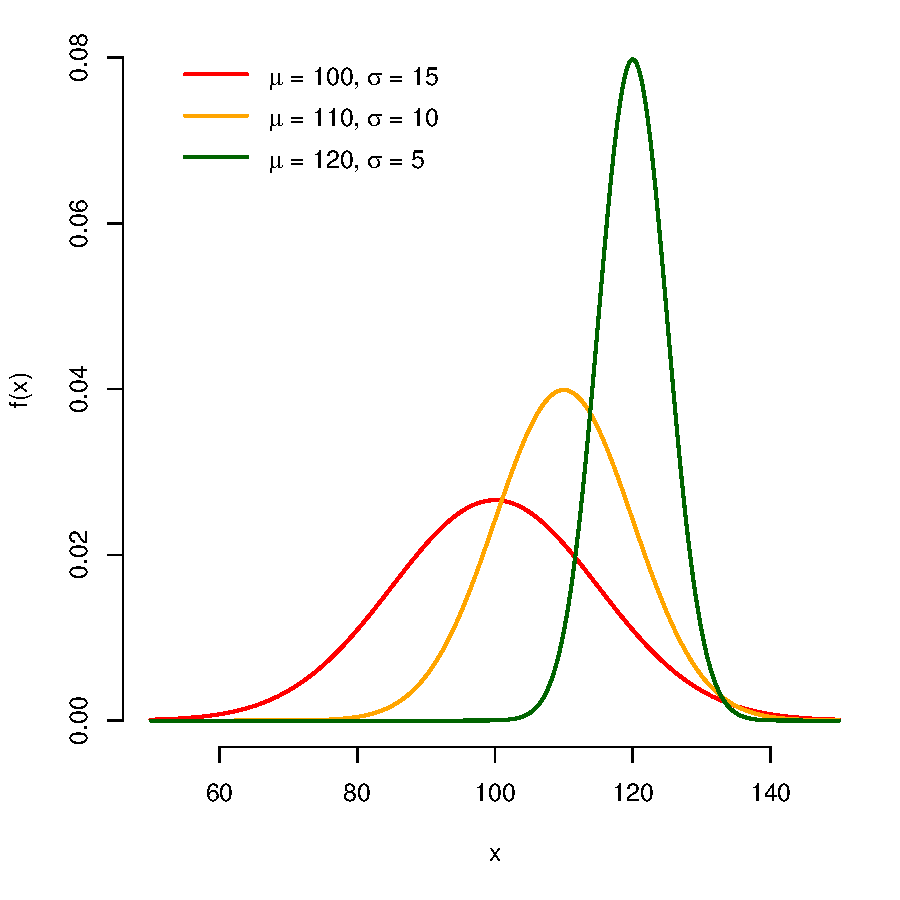
\includegraphics[width=.6\linewidth]{img/ukazka-obr02.pdf}
% \caption{A figure with a plot, not entirely related to anything. If you copy the figures from anywhere, always refer to the original author, ideally by citation (if possible). In particular, this picture --- and many others, also a lot of surrounding code --- was taken from the example bachelor thesis of MFF, originally created by Martin Mareš and others.}
% \label{fig:g}
% \end{figure}

% \begin{figure}
% \centering
% \tikzstyle{box}=[rectangle,draw,rounded corners=0.5ex,fill=green!10]
% \begin{tikzpicture}[thick,font=\sf\scriptsize]
% \node[box,rotate=45] (a) {A test.};
% \node[] (b) at (4,0) {Node with no border!};
% \node[circle,draw,dashed,fill=yellow!20, text width=6em, align=center] (c) at (0,4) {Ugly yellow node.\\Is this the Sun?};
% \node[box, right=1cm of c] (d) {Math: $X=\sqrt{\frac{y}{z}}$};
% \draw[->](a) to (b);
% \draw[->](a) to[bend left=30] node[midway,sloped,anchor=north] {flow flows} (c);
% \draw[->>>,dotted](b) to[bend right=30] (d);
% \draw[ultra thick](c) to (d);

% \end{tikzpicture}
% \caption{An example diagram typeset with TikZ.}
% \label{fig:schema}
% \end{figure}

% \begin{algorithm}
% \begin{algorithmic}
% \Function{ExecuteWithHighProbability}{$A$}
% 	\State $r \gets$ a random number between $0$ and $1$
% 	\State $\varepsilon \gets 0.0000000000000000000000000000000000000042$
% 	\If{$r\geq\varepsilon$}
% 		\State execute $A$ \Comment{We discard the return value}
% 	\Else
% 		\State print: \texttt{Not today, sorry.}
% 	\EndIf
% \EndFunction
% \end{algorithmic}
% \caption{Algorithm that executes an action with high probability. Do not care about formal semantics in the pseudocode --- semicolons, types, correct function call parameters and similar nonsense from `realistic' languages can be safely omitted. Instead make sure that the intuition behind (and perhaps some hints about its correctness or various corner cases) can be seen as easily as possible.}
% \label{alg:w}
% \end{algorithm}

% \section{Extra typesetting hints}

% Do not overuse text formatting for highlighting various important parts of your sentences. If an idea cannot be communicated without formatting, the sentence probably needs rewriting anyway. Imagine the thesis being read aloud as a podcast --- the storytellers are generally unable to speak in boldface font.

% Most importantly, do \underline{not} overuse bold text, which is designed to literally \textbf{shine from the page} to be the first thing that catches the eye of the reader. More precisely, use bold text only for `navigation' elements that need to be seen and located first, such as headings, list item leads, and figure numbers.

% Use underline only in dire necessity, such as in the previous paragraph where it was inevitable to ensure that the reader remembers to never typeset boldface text manually again.

% Use \emph{emphasis} to highlight the first occurrences of important terms that the reader should notice. The feeling the emphasis produces is, roughly, ``Oh my --- what a nicely slanted word! Surely I expect it be important for the rest of the thesis!''

% Finally, never draw a vertical line, not even in a table or around figures, ever. Vertical lines outside of the figures are ugly.

\chapter{Popis vstupných dát a ich spracovanie}
\label{chap:ThirdChapter}
You should have a separate chapter for presenting your results (generated by the stuff described previously, in our case in \cref{chap:math}). Remember that your work needs to be validated rigorously, and no one will believe you if you just say that `it worked well for you'.

Instead, try some of the following:
\begin{itemize}
\item State a hypothesis and prove it statistically
\item Show plots with measurements that you did to prove your results (e.g. speedup). Use either \texttt{R} and \texttt{ggplot}, or Python with \texttt{matplotlib} to generate the plots.\footnote{Honestly, the plots from \texttt{ggplot} look \underline{much} better.} Save them as PDF to avoid printing pixels (as in \cref{fig:f}).
\item Compare with other similar software/theses/authors/results, if possible
\item Show example source code (e.g. for demonstrating how easily your results can be used)
\item Include a `toy problem' for demonstrating the basic functionality of your approach and detail all important properties and results on that
\item Include clear pictures of `inputs' and `outputs' of all your algorithms, if applicable
% \end{itemize}

% \begin{figure}
% \centering
% 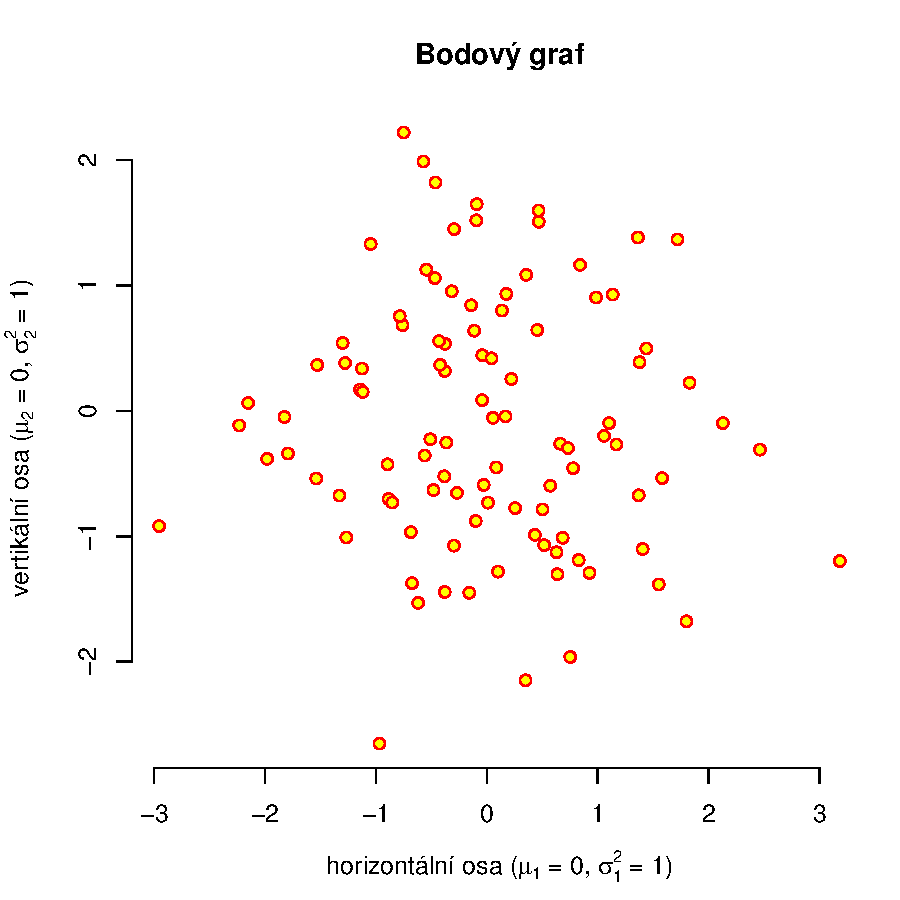
\includegraphics[width=.6\linewidth]{img/ukazka-obr01.pdf}
% \caption{This caption is a friendly reminder to never insert figures ``in text,'' without a floating environment, unless explicitly needed for maintaining the text flow (e.g., the figure is small and developing with the text, like some of the centered equations, as in \cref{thm:y}). All figures \emph{must} be referenced by number from the text (so that the readers can find them when they read the text) and properly captioned (so that the readers can interpret the figure even if they look at it before reading the text --- reviewers love to do that).}
% \label{fig:f}
% \end{figure}

% It is sometimes convenient (even recommended by some journals, including Cell) to name the results sub-sections so that they state what exactly has been achieved. Examples follow.

% \section{SuperProgram is faster than OldAlgorithm}
% \subsection{Scalability estimation}
% \subsection{Precision of the results}
% \section{Weird theorem is proven by induction}
% \section{Amount of code reduced by CodeRedTool}
% \subsection{Example}
% \subsection{Performance on real codebases}
% \section{\sloppy NeuroticHelper improves neural network learning}

% \section{Graphics and figure quality}

% No matter how great the text content of your thesis is, the pictures will always catch the attention first. This creates the very important first impression of the thesis contents and general quality. Crucially, that also decides whether the thesis is later read with joy, or carefully examined with suspicion.

% Preparing your thesis in a way such that this first impression gets communicated smoothly and precisely helps both the reviewer and you: the reviewer will not have a hard time understanding what exactly you wanted to convey, and you will get a better grade.

% Making the graphics `work for you' involves doing some extra work that is often unexpected. At the same time, you will need to fit into graphics quality constraints and guidelines that are rarely understood before you actually see a bad example. As a rule of thumb, you should allocate at least the same amount of time and effort for making the figures look good as you would for writing, editing and correcting the same page area of paragraph text.

% \subsection{Visualize all important ideas}
% The set of figures in your thesis should be comprehensive and complete. For all important ideas, constructions, complicated setups and results there should be a visualization that the reader can refer to in case the text does not paint the `mental image' sufficiently well. At the bare minimum, you should have at least 3 figures (roughly corresponding to the 3 chapters) that clearly and unambiguously show:
% \begin{enumerate}
% \item the context of the problem you are solving, optionally with e.g.~question marks and exclamation marks placed to highlight the problems and research questions
% \item the overall architecture of your solution (usually as a diagram with arrows, such as in \cref{fig:schema}, ideally with tiny toy examples of the inputs and outputs of each box),
% \item the advancement or the distinctive property of your solution, usually in a benchmark plot, or as a clear demonstration and comparison of your results.
% \end{enumerate}

% \subsection{Make the figures comprehensible}
% The figures should be easily comprehensible. Surprisingly, that requires you to follow some common ``standards'' in figure design and processing. People are often used to a certain form of the visualizations, and (unless you have a very good reason) deviating from the standard is going to make the comprehension much more complicated. The common standards include the following:
% \begin{itemize}
%   \item caption everything correctly, place the caption at an expectable position
%   \item systematically label the plots with `main' titles (usually in boldface, above the plot), plot axes, axis units and ticks, and legends
%   \item lay out the diagrams systematically, ideally follow a structure of a bottom-up tree, a left-to-right pipeline, a top-down layered architecture, or a center-to-borders mindmap
%   \item {use colors that convey the required information correctly \par\footnotesize Although many people carry some intuition for color use, achieving a really correct utilization of colors is often very hard without previous experience in color science and typesetting. Always remember that everyone perceives color hues differently, therefore the best distinction between the colors is done by varying lightness of the graphics elements (i.e., separating the data by dark vs.~light) rather than by using hues (i.e., forcing people to guess which one of salmon and olive colors means ``better''). Almost 10\% of the population have their vision impaired by some form of color vision deficiency, most frequently by deuteranomaly that prevents interpretation of even the most `obvious' hue differences, such as green vs.~red. Finally, printed colors look surprisingly different from the on-screen colors. You can prevent much of these problems by using standardized palettes and well-tested color gradients, such as the ones from ColorBrewer\footnote{\url{https://colorbrewer2.org}} and ViridisLite\footnote{\url{https://sjmgarnier.github.io/viridisLite/}}. Check if your pictures still look good if converted to greyscale, and use a color deficiency simulator to check how the colors are perceived with deuteranomaly.}
% \end{itemize}

% Avoid large areas of over-saturated and dark colors:
% \begin{itemize}
%   \item under no circumstances use dark backgrounds for any graphical elements, such as diagram boxes and tables --- use very light, slightly desaturated colors instead
%   \item avoid using figures that contain lots of dark color (as a common example, heatmaps rendered with the `magma' color palette often look like huge black slabs that are visible even through the paper sheet, thus making a dark smudge on the neighboring page)
%   \item increase the brightness of any photos to match the average brightness of the text around the figure
% \end{itemize}

% Remember to test your figures on other people --- usually, just asking `What do you think the figure should show?' can help you debug many mistakes in your graphics. If they think that the figure says something different than what you planned, then most likely it is your figure what is wrong, not the understanding of others.

% Finally, there are many magnificent resources that help you arrange your graphics correctly. The two books by Tufte~\cite{tufte1990envisioning,tufte1983visual} are arguably classics in the area. Additionally, you may find many interesting resources to help you with technical aspects of plotting, such as the \texttt{ggplot}-style `Fundamentals' book by~\citet{wilke2019fundamentals}, and a wonderful manual for the TikZ/PGF graphics system by~\citet{tantau2015tikz} that will help you draw high-quality diagrams (like the one in~\cref{fig:schema}).

% \section{What is a discussion?}
% After you present the results and show that your contributions work, it is important to \emph{interpret} them, showing what they mean in the wider context of the thesis topic, for the researchers who work in the area, and for the more general public, such as for the users.

% Separate discussion sections are therefore common in life sciences where some ambiguity in result interpretation is common, and the carefully developed intuition about the wider context is sometimes the only thing that the authors have. Exact sciences and mathematicians do not need to use the discussion sections as often. Despite of that, it is nice to position your output into the previously existing environment, answering:
% \begin{itemize}
% \item What is the potential application of the result?
% \item Does the result solve a problem that other people encountered?
% \item Did the results point to any new (surprising) facts?
% \item How (and why) is the approach you chose different from what the others have done previously?
% \item Why is the result important for your future work (or work of anyone other)?
% \item Can the results be used to replace (and improve) anything that is used currently?
% \end{itemize}

% If you do not know the answers, you may want to ask the supervisor. Also, do not worry if the discussion section is half-empty or completely pointless; you may remove it completely without much consequence. It is just a bachelor thesis, not a world-saving avenger thesis.

\chapter{Proces detekcie anonymizovaných častí dokumentov}
\label{chap:FourthChapter}
\chapter{Vizualizácia výsledkov}
\label{chap:FifthChapter}
\begin{hyphenrules}{nohyphenation}
%\todo[inline]{bez nadpisu... potom skuste obrazkom pridat okraj, aby bolo jasne, aka velka stranka je}
Keďže obsahom práce je niečo, čo je veľmi jednoducho vizualizovateľné, a to jednoduchým porovnaním vstupov a výstupov, v ďalšej podkapitole je uvedených niekoľko príkladov. Uvedieme príklady z testovacieho datasetu a aj niekoľko iných dokumentov, ktoré pouvažujeme za zaujímavé na zhodnotenie. Ku každému príkladu uvedieme komentár.
\section{Interpretácia získaných štatistík}
Dosiahnuté výstupné detegované oblasti prezentujeme s dôrazom na~to, ako tieto dáta ovplyvňujú celkové pochopenie problému a efektivitu riešenia. Pre prehľadnosť uvedieme len vybrané strany dokumentov, nakoľko väčšina dokumentov je viacstranová a nie na každej strane sa objavuje anonymizovaná oblasť. Vľavo budeme uvádzať vstup, vpravo výstup.
\newline 

Ako prvé uvedieme príklady, kde detekcia funguje správne podľa očakávaní. Na ďalšej strane na obrázku \ref{fig:5.1} môžeme vidieť, že na dokumentoch, kde bol použitý typ anonymizácie čierny obdĺžník, náš algoritmus presne deteguje tieto miesta.

\begin{figure}[H]
\begin{minipage}[t]{.5\linewidth}
\fbox{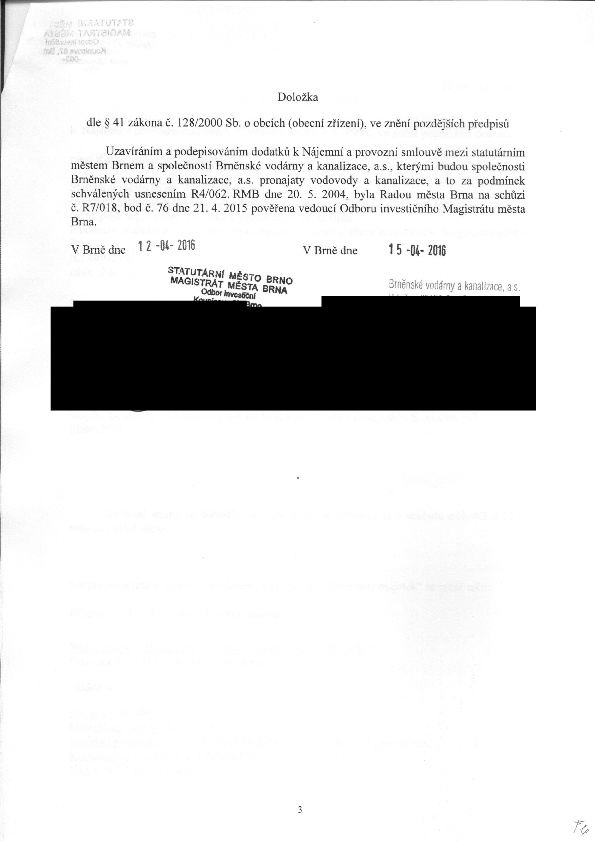
\includegraphics[width=0.9\linewidth]{img/5/03_original.jpg}}
\caption{Percento anonymizovania : 10,61 \%}
\label{fig:5.1} 
\end{minipage}\hfill
\begin{minipage}[b]{.5\linewidth}
\fbox{
\includegraphics[width=0.9\linewidth]{img/5/03_result.jpg}}
\end{minipage}
\end{figure}

Za zmienku tu stojí všimnúť si ľavý horný roh, kde sa vyskytuje relatívne tmavý trojuholník, ktorý vznikol nedokonalým priložením papiera na skener. Náš algoritmus v tomto prípade správne detegoval len miesto, ktoré je naozaj začiernené. Môžeme si všimnúť komplexitu začiernenej plochy. Nejedná sa o~štvoruholník, ale o viac komplexný tvar. V prípade použitia prístupu detekcie bounding boxov by sme museli počítať s tým, že by bol bounding box väčší a~zahŕňal by aj miesta, ktoré začiernené nie sú. To by znamenalo viac algoritmickej práce na overenie, že bounding box naozaj obsahuje len tú plochu, ktorú má a~v~takomto prípade by bolo potrebné rozparcelovať bounding boxy tak, aby dokonale obkreslili nepravidelné tvary. Problém s použitím prístupu bounding boxov by bol ešte viac viditeľný, ak by bola na vstupnom obraze šikmá anonymizovaná oblasť, ako môžeme vidieť v ďalšom príklade na obr. \ref{fig:5.2}.

\begin{figure}[H]
\begin{minipage}[t]{.5\linewidth}
\fbox{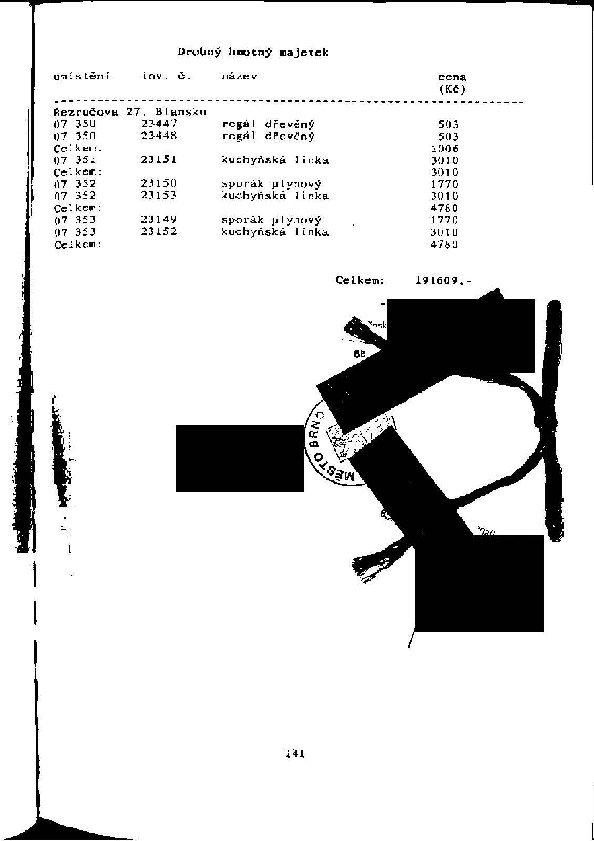
\includegraphics[width=0.9\linewidth]{img/5/73_original.jpg}}
\caption{Percento anonymizovania : 12,68 \%}
\label{fig:5.2} 
\end{minipage}\hfill
\begin{minipage}[b]{.5\linewidth}
\fbox{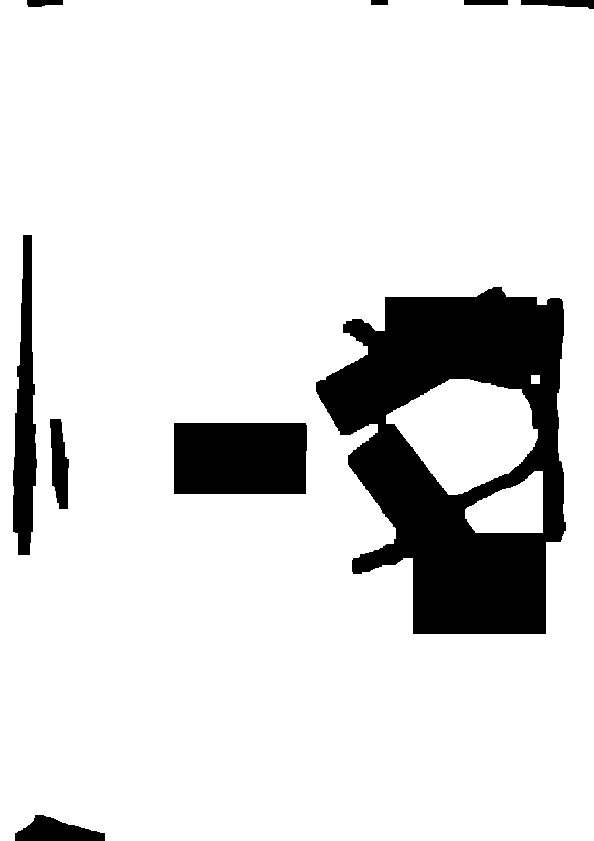
\includegraphics[width=0.9\linewidth]{img/5/73_result.jpg}}
\end{minipage}
\end{figure}

V tomto prípade sa jedná o dokument z roku 1994 a môžeme si všimnúť, že to je nekvalitný sken. V tomto prípade je zobrazená posledná strana a vzhľadom na použitý algoritmus je vidieť, že za anonymizovanú oblasť boli detegované aj oblasti, ktoré nimi reálne nie sú. V tomto konkrétnom príklade bolo pre použitý algoritmus obtiažne rozlíšiť medzi nedokonalosťami skenu, zväzujúcou šnúrkou a najskôr nálepkami prekrývajúce dôležité informácie tohto dokumentu. 
\newline

Jedným z možných riešení by bola detekcia zvislých pozdĺžnych oblastí a~tie vyhodnocovať za chybu. Pri implementácii sme premýšľali nad možnosťami filtrácie, no v tej dobe sme nemohli prísť s rozumným riešením, ktoré by nemalo fatálny dopad na iné analyzované dokumenty, ako si ukážeme na ďalšej strane, na obr. \ref{fig:5.3}.

\begin{figure}[H]
\begin{minipage}[t]{.5\linewidth}
\fbox{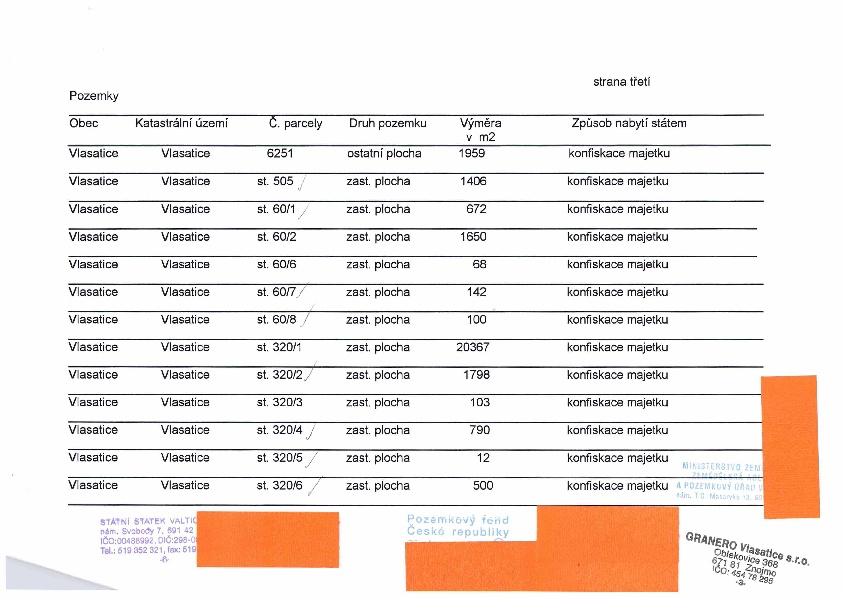
\includegraphics[width=0.9\linewidth]{img/5/9_original.jpg}}
\caption{Percento anonymizovania : 7,45 \%}
\label{fig:5.3} 
\end{minipage}\hfill
\begin{minipage}[b]{.5\linewidth}
\fbox{
\includegraphics[width=0.9\linewidth]{img/5/9_result.jpg}}
\end{minipage}
\end{figure}

V tomto prípade sa jedná o prelepenie farebnými nálepkami, ktoré algoritmus rovnako dokázal detegovať a správne určiť za anonymizovanú oblasť. 
\newline

Na predchádzajúcom príklade sme spomenuli možnú filtráciu pozdĺžnych nepravidelných objektov, čo by v tomto prípade znamenalo detekciu oblasti vpravo od tabuľky (všimnime si, že oblasť nie je zarovnaná a je šikmo) a po následnej filtárcii by došlo k odstráneniu oblasti, ktorá bola pôvodne detegovaná správne. 
\newline

Znovu si môžeme všimnúť celkom výrazného trojuholníka v ľavom dolnom rohu, ktorý náš algoritmus dokázal odfiltrovať a nevyhodnotiť ako tmavú plochu, čo by spôsobilo nesprávne označenie oblasti za anonymizovanú.

\begin{figure}[H]
\begin{minipage}[t]{.4\linewidth}
\fbox{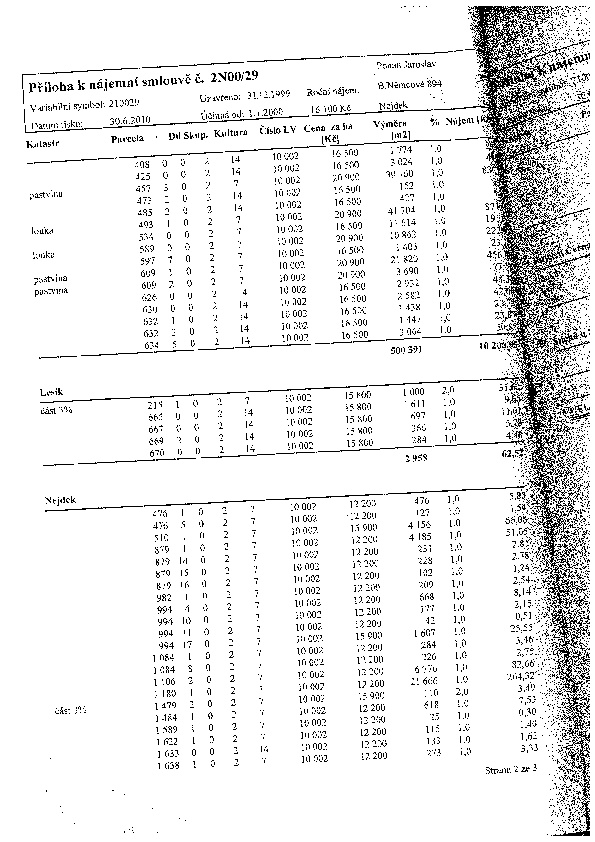
\includegraphics[width=0.9\linewidth]{img/5/4_original.jpg}}
\caption{Percento anonymizovania : 0,08 \%}
\label{fig:5.4} 
\end{minipage}\hfill
\begin{minipage}[b]{.4\linewidth}
\fbox{
\includegraphics[width=0.9\linewidth]{img/5/4_result.jpg}}
\end{minipage}
\end{figure}

Na obrázku \ref{fig:5.4} vidíme ďalšiu stranu z dokumentu, ktorý bol skenovaný veľmi nekvalitne. V origináli sa síce nevyskytuje anonymizovaná oblasť, no kvôli veľmi zlému skenu boli niektoré oblasti dostatočne tmavé na to, aby boli vyhodnotené naším algoritmom za anonymizované oblasti. Nejedná sa o veľké plochy a možné riešenie takýchto anomálií popisujeme v záverečnej kapitole \ref{chap:conclusion}.
\newline

Na posledných príkladoch si ukážeme tzv. false positives, ktoré algoritmus nebol schopný rozoznať a správne odfiltrovať.

\begin{figure}[H]
\begin{minipage}[t]{.5\linewidth}
\fbox{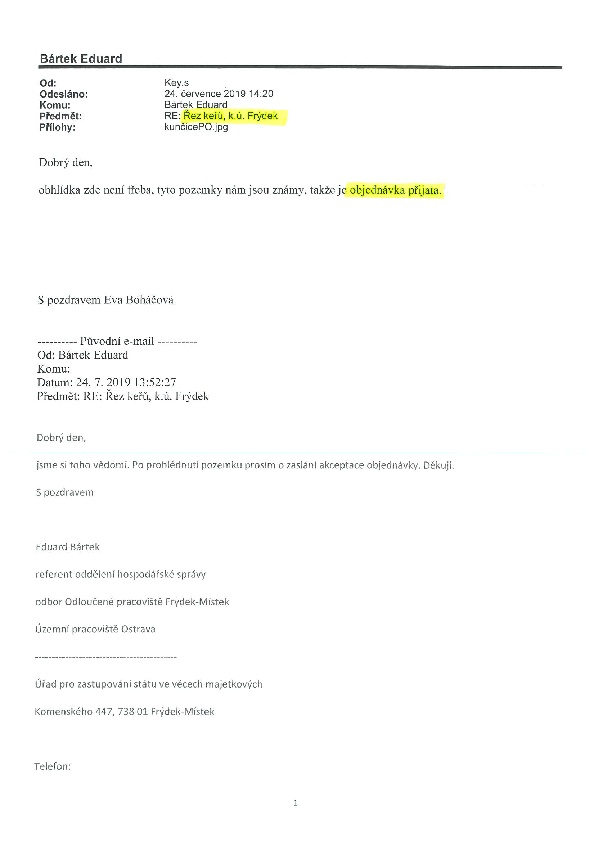
\includegraphics[width=0.9\linewidth]{img/5/3_original.jpg}}
\caption{Percento anonymizovania : 0,07 \%}
\label{fig:5.5} 
\end{minipage}\hfill
\begin{minipage}[b]{.5\linewidth}
\fbox{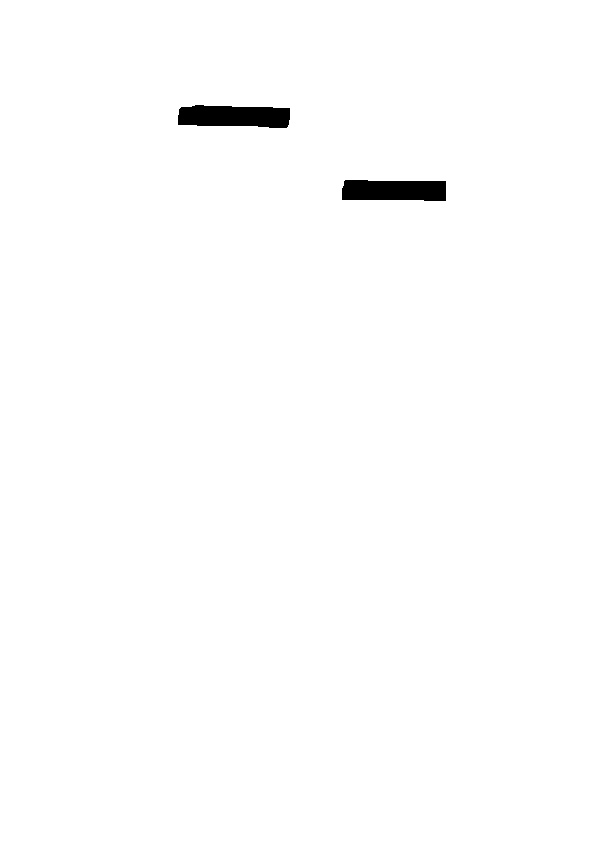
\includegraphics[width=0.9\linewidth]{img/5/3_result.jpg}}
\end{minipage}
\end{figure}

Ako bolo spomenuté v popise algoritmu v \ref{chap:4.1.2}, v prípade detekcie farebných pixelov berieme tieto pixely ako možné anonymizované oblasti. V tomto prípade sa však jedná o zvýrazňovač, no algoritmus to vyhodnotil ako anonymizovanú plochu, a teda tieto oblasti sú false positive. Možné riešenia a prístupy sú spomenuté v záverečnej kapitole \ref{chap:conclusion}.
\newline

Na obrázku \ref{fig:5.6} vidíme obdobný problém, tentokrát týkajúci sa úradnej pečiatky, ktorá je výrazná červená. 

\begin{figure}[H]
\begin{minipage}[t]{.4\linewidth}
\fbox{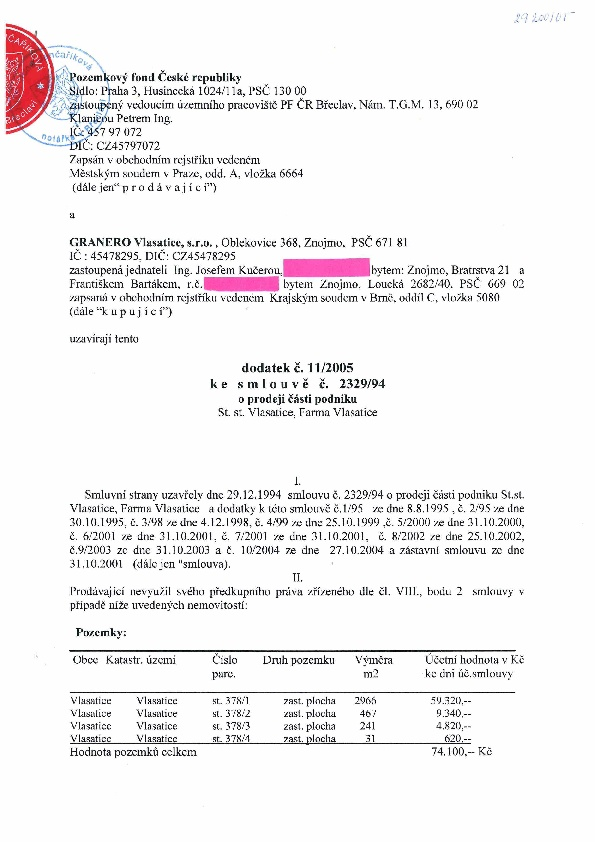
\includegraphics[width=0.9\linewidth]{img/5/1_original.jpg}}
\caption{Percento anonymizovania : 1,4 \%}
\label{fig:5.6} 
\end{minipage}\hfill
\begin{minipage}[b]{.4\linewidth}
\fbox{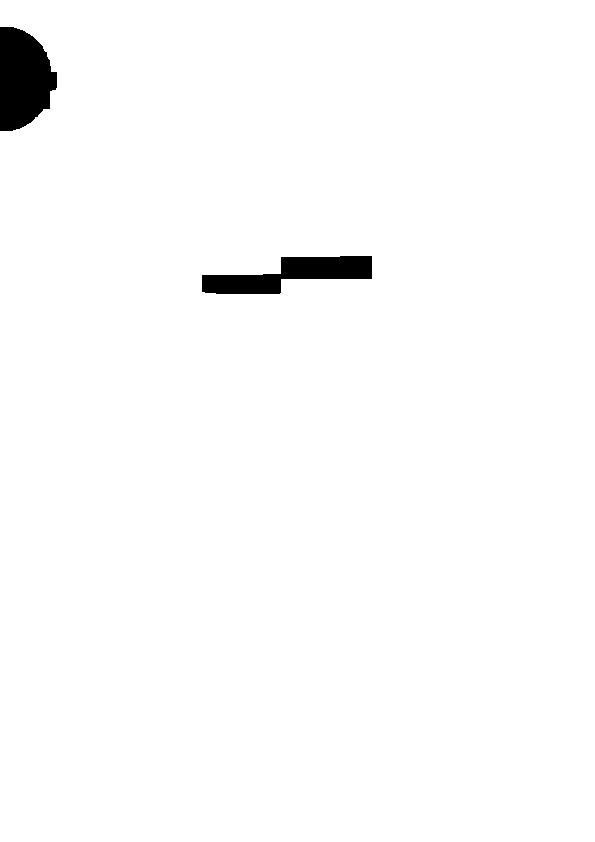
\includegraphics[width=0.9\linewidth]{img/5/1_result.jpg}}
\end{minipage}
\end{figure}

Posledný príklad, ktorý uvedieme (obr. \ref{fig:5.7}), je detekcia anonymizovaných oblastí šumom. Tento typ anonymizácie bol jednym z hlavných problémov, nakoľko bolo veľmi ťažké správne vyfiltrovať bežný šum, ktorý vznikal pri zlom skene od šumu, ktorý prekrýval nejaké údaje a teda sa jednalo o anonymizovanú oblasť. Detegované oblasti nie sú dokonalé, každopádne môžeme prehlásiť, že aj takýto typ anonymizácie sme schopní detegovať a relatívne presne označiť.


\begin{figure}[H]
\begin{minipage}[t]{.4\linewidth}
\fbox{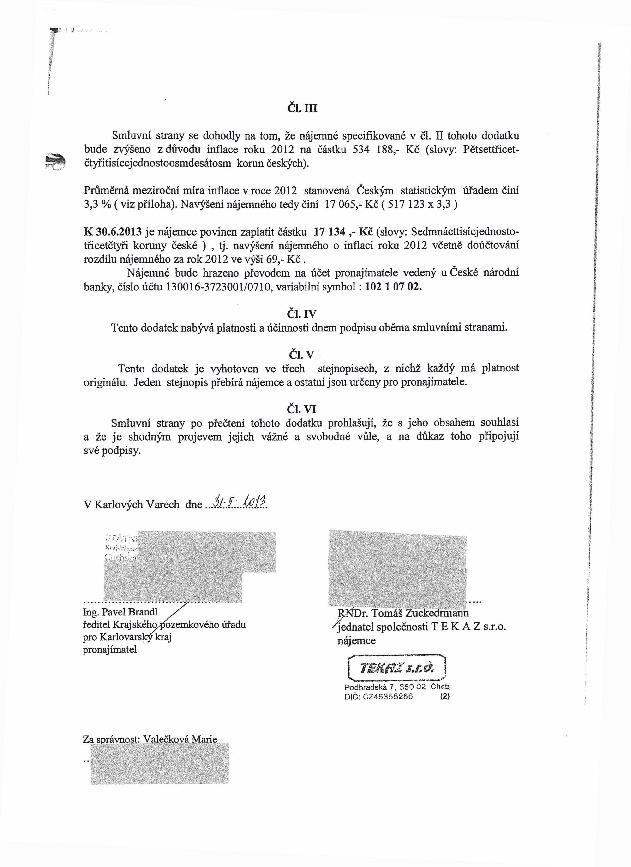
\includegraphics[width=0.9\linewidth]{img/5/2_original.jpg}}
\caption{Percento anonymizovania : 4,2 \%}
\label{fig:5.7} 
\end{minipage}\hfill
\begin{minipage}[b]{.4\linewidth}
\fbox{
\includegraphics[width=0.9\linewidth]{img/5/2_result.jpg}}
\end{minipage}
\end{figure}

\subsection{Dopady na ďalší vývoj}
Na základe vykonaných pozorovaní a analýz detegovaných oblastí je zrejmé, že algoritmus má schopnosť identifikovať anonymizované oblasti s vysokou presnosťou, zároveň však sledujeme výzvy v špecifických scenároch, ktoré vyžadujú ďalšie vylepšenia. Niekoľko kľúčových poznatkov a návrhov pre ďalší význam, ktoré uvádzame, sú:
\begin{enumerate}
    \item Zlepšenie filtrovacích metód. 
    
    Ako sme si mohli všimnúť v príkladoch s nekvalitnými skenmi, algoritmus má tendenciu označovať tmavé zašumené oblasti za anonymizované. Pre budúci vývoj tak predpokladáme implementáciu pokročilých filtrovacích techník, ktoré by boli schopné dokázať lepšie rozlišovať medzi skutočne anonymizovanými oblasťami a nedokonalosťami skenu.
    \item Rozpoznávanie kontextu. 
    
    Ďalší vývoj algoritmu by mal cieliť na identifikáciu vzorov, kde dochádza k~anonymizácii častejšie a naopak miesta, kde sa anonymizácia spravidla nevyskytuje (napr. okraje strán, nadpisy, určité formáty textov...).

    \item Optimalizácia detekcie tvarov.

    Algoritmus často nesprávne označí zvýrazňovače či farebné pečiatky ako anonymizované oblasti. Budúci vývoj by mal zahrnúť detekciu takýchto tvarov a správne ich identifikovať a ignorovať.
\end{enumerate}
\end{hyphenrules}
\chapter{Implementácia riešenia}
\label{chap:SixthChapter}
\section{Výber technológií a nástrojov}
\subsection{Kritériá výberu}
\begin{hyphenrules}{nohyphenation}
Rozhodnutie pri výbere technológie padlo na \texttt{C\#} a \texttt{.NET 8} kvôli robustnej podpore pre webové služby a~pokročilým vedomostiam daného jazyka. Pre analýzu a~spracovanie PDF dokumentov boli použité knižnice \texttt{ImageMagick} a~\texttt{OpenCV}. Náš softvér cieli na operačný system Windows 10.

\subsection{Použité technológie}
\begin{itemize}
    \item Jazyk: \texttt{C\#}
    \item Framework: \texttt{.NET 8}
    \item API: Minimal API v \texttt{.NET 8}
    \item Použité knižnice (NuGety): 
    \begin{itemize}
        \item Coverlet \cite{coverlet}
        
        - Použitý pre štatistiku nad pokrytím kódu testami.
        \item ErrorOr \cite{error-or}
        
        - Menší NuGet, ktorý pomáha riešiť vyhadzovanie výnimiek a miesto nich poskytuje intuitívny prístup k návratovej hodnote.
        \item FluentValidation \cite{fluentvalidation}

        - Intuitívny spôsob validácie vstupov a validácie pri tvorbe objektov.
        \item Magick.NET \cite{magicknet}

        - Nadstavba nad ImageMagick, vhodný pri manipulácii a úprave obrázkov, v našom prípade použitý pri konverzii PDF dokumentov do formátu vhodného pre ďalšie procesy.
        \item Mapster \cite{mapster}

        - Umožňuje jednoduché mapovanie objektov, primárne použitý pri mapovaní HTTP requestov na objekty, s ktorými ďalej pracuje aplikácia.
        \item MediatR \cite{mediatr}

        - Umožňuje implementáciu vzoru mediátora, čím zjednodušuje komunikáciu medzi komponentami aplikácie tým, že sprostredkováva požiadavky a notifikácie medzi odosielateľmi a prijímateľmi bez ich vzájomnej závislosti.

        \item Entity Framework Core \cite{efcore}

        - ORM knižnica pre .NET, ktorá umožňuje pracovať s databázami, umožňuje mapovanie medzi databázovými tabuľkami a triedami v~aplikácii.

        \item Microsoft DependencyInjection \cite{dependency-injection}

        - Poskytuje vstavanú podporu pre Dependency Injection, umožňuje automatickú správu závislostí medzi jednotlivými komponentami aplikácie.

        \item OpenCvSharp4 \cite{opencv}

        - Nadstavba nad OpenCV pre .NET.

        \item xUnit \cite{xunit}

        - Testovací framework slúžiaci na jednoduché testovanie aplikácie.
        
    \end{itemize}
\end{itemize}

Aplikácia je vybavená aj SQLite\cite{sqlite} databázou, ktorá poskytuje ľahkú a~kompaktnú relačnú databázu a umožňuje lokálne ukladanie a spracovanie dát bez potreby samostatného servera.

\section{Architektúra a dizajn systému}
\subsection{Architektúra riešenia}
Architektúra našej aplikácie je založená na tzv. Domain-Driven Design, ktorá je popísana v knihe od Scotta Millett-a a Nicka Tune-a, \textit{Patterns, Principles, and Practices of Domain-Driven Design}\cite{millett2015ddd}. Domain-Driven Design (DDD), resp. Domain-Driven architecture je často označovaný aj ako vrstvová architektúra, cibuľová architektúra či "čistá" architektúra. 
\newline

Vrstvová architektúra je rozdelená do viacerých vrstiev, ktoré sa vzťahujú na~rozličné aspekty daného systému. Každá vrstva má jasnú a~špecifickú úlohu a~vrstvy sa navzájom ovplyvňujú len jedným smerom.

Hlavnými prvkami vrstvovej architektúry sú:
\begin{enumerate}
    \item Prezenčná vrstva: Zodpovedá za interakciu s uživateľom,
    \item Aplikačná vrstva: Zodpovedá za implementáciu biznisovej logiky, ktorá sa vzťahuje na uživateľské požiadavky,
    \item Servisná vrstva: Slúži na poskytovanie služieb, ktoré sú potrebné pre aplikáciu,
    \item Infraštruktúrna vrstva: Zodpovedá za správu a komunikáciu s externými zdrojmi,
    \item Perzistentná vrstva: Slúži na komunikáciu s perzistentne uloženými dátami, databázou.
\end{enumerate}


\begin{figure}[H]
    \centering
    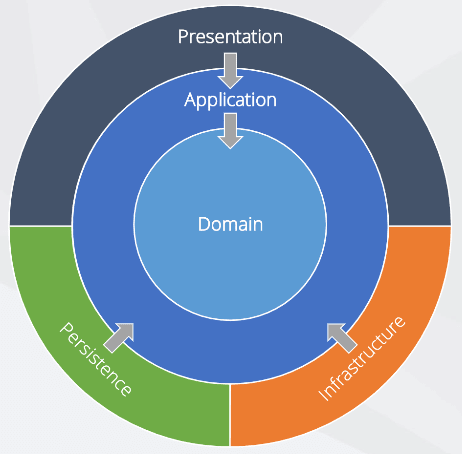
\includegraphics[width=0.4\linewidth]{img/onion.png}
    \caption{Grafické znázornenie cibuľovej architektúry\cite{danielrusnok}}
    \label{fig:6.1}
\end{figure}
Každá vrstva je navrhnutá tak, aby bola izolovaná od ostatných vrstiev. Vrstvy medzi sebou komunikujú pomocou rozhraní a preto zmeny v jednej vrstve nevytvárajú nepredvídateľné zmeny v iných vrstvách. Pomocou rozhraní definujeme, čo dané vrstvy môžu a nemôžu robiť.
\newline

Najväčšími výhodami tejto architektúry sú modularita, odolnosť voči zmenám a jednoduchosť pri návrhu samotnej aplikácie.

\section{Detaily implementácie}

\subsection{Pomocné aplikácie a testovacie projekty}
\label{chap:6.3.1}
V rámci projektu DAPP\cite{lukassalak} sme implementovali pomocný projekt s~názvom \texttt{ManualCheckerUtility}. Pri spustení automaticky stiahne dokumenty, ktoré sú následne po jednotlivých stránkach zobrazované uživateľovi. V pravej strane sa nachádza niekoľko možností, ktoré užívateľ môže zvoliť a tie sa následne postupne ukladajú do štatistiky. 

\begin{figure}[H]
    \centering
    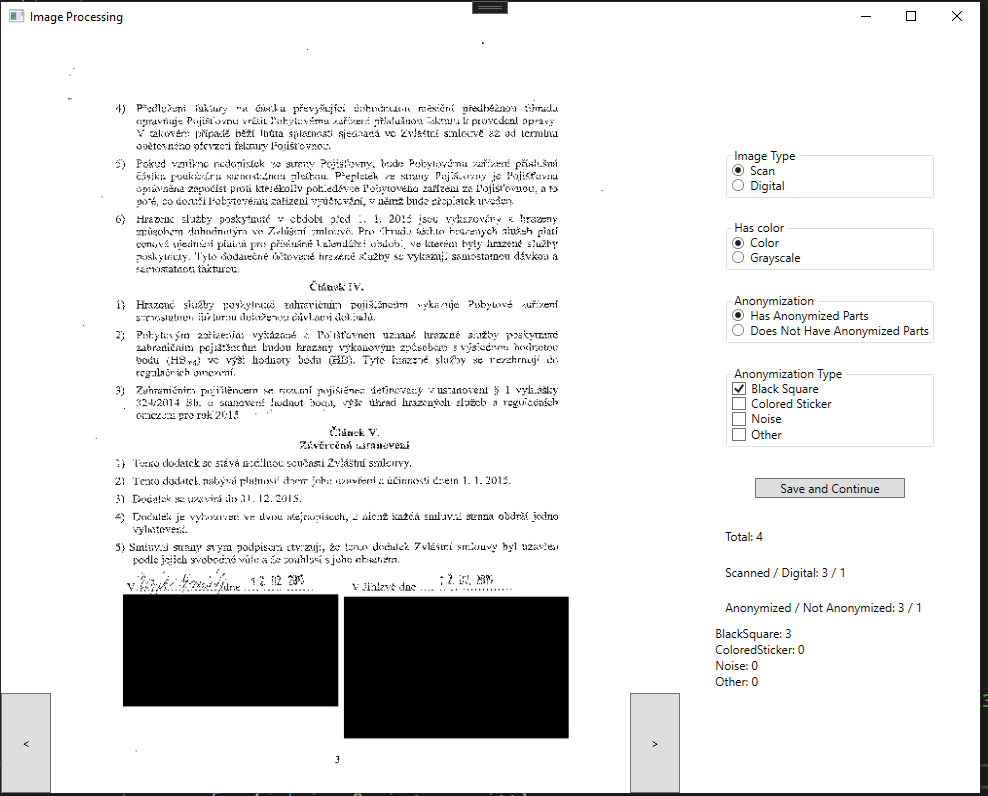
\includegraphics[width=0.9\linewidth]{img/image_proc.png}
    \caption{Ukážka grafického rozhrania \texttt{ManualCheckerUtility}}
    \label{fig:6.2}
\end{figure}

Súčasťou riešenia okrem testov je aj projekt s~názvom \texttt{GenerateTestResults}. Jedná sa o jednoduchý skript, ktorý umožňuje rýchlo generovať výsledky s~aktuálnym kódom a ukladať tieto výsledky sekvenčne s prebiehajúcimi zmenami. 
Skript si na začiatku vytvorí WebClient hlavného programu nesúceho názov API2. API2 je druhá verzia projektu API, ktorá bola vzhľadom na použitú architektúru zastaraná a preto sme sa rozhodli prejsť na tzv. minimal api \cite{aspnetcore}. Následne po inicializácii WebClient-a prevoláva toto API s requestami obsahujúcimi jednotlivé dokumenty z našej testovacej sady. Po vrátení response sa tieto dáta dekomponujú z~formátu JSON a uložia na disk, kde ich je potom možné prehliadať. Ukladajú sa originálne snímky, analyzované snímky a percentá anonymizácie pre jednotlivé strany.

\subsection{Realizácia algoritmu}
Hlavným projektom, ktorý je nosnou časťou našej aplikácie okrem samotného API a jeho častí, je projekt s názvom \texttt{DAPPAnalyzer}, ktorý obsahuje algoritmus na detekciu anonymizovaných častí.
\newline

Súbor \texttt{PDFAnalyzer.cs} obsahuje implementáciu triedy \texttt{PDFAnalyzer}, ktorá implementuje niekoľko metód. Hlavnou a vstupnou metódou je metóda \texttt{Task<AnalyzedResult> AnalyzeAsync(DappPDF pdf);}, ktorá je jedinou verejnou metódou tejto triedy. Jej funkciou je paralelne pre každú stranu z~parametru pustiť privátnu funkciu \texttt{AnalyzePage} a následne vrátené výsledky uložiť do modelu \texttt{AnalyzedResult}, ktorý obsahuje okrem identifikačných znakov, akými sú názov dokumentu, url či počet strán dokumentu, samotné výsledky analýzy. Tými sú:
\begin{itemize}
    \item \texttt{containsAnonymizedData} : boolean, ktorý určuje, či boli detegované anonymizované oblasti,
    \item \texttt{anonymizedPercentagePerPage} : slovník, kde kľúč je index strany a~hodnota je percento anonymizácie pre danú stranu,
    \item \texttt{originalImages} : slovník, kde kľúč je index strany a hodnota je \texttt{byte[]}, teda snímok danej strany uložený ako \texttt{byte array},
    \item \texttt{anonymizedImages} : rovnako ako pri \texttt{originalImages}, až na to, že \texttt{byte[]} obsahuje výslednú "masku", teda obraz, kde sú znázornené len anonymizované oblasti.
    
\end{itemize}

Na ďalšej strane prikladáme zdrojový kód tejto funkcie. Pre ešte bližšie detaily prikladáme v prílohe zdrojový kód, kde je dostupná celá implementácia so všetkými pomocnými skriptami a testovacími súbormi.
\newpage
\begin{lstlisting}
internal static Mat GetAnonymizedParts(
    Mat img, 
    int erodeValue = 8, 
    int dilateValue = 4)
{

    var coloredPixels = ColoredPixels(img);
    // Increase their saturation 
    var imgSaturatedColors = img;
    if (coloredPixels.Count != 0)
    {
       imgSaturatedColors = 
            IncreaseSaturation(img, coloredPixels, 100);
    }
    // Create structuring element
    Mat se = 
        Cv2.GetStructuringElement(
            MorphShapes.Rect, 
            new Size(3, 3));
    var dilated = Dilate(imgSaturatedColors, se);

    var dilated_threshold = Threshold(dilated, 20);
    var dilated2 = Dilate(dilated_threshold, se);


    var result = dilated2;
    for (int i = 0; i < erodeValue; i++)
    {
        result = Erode(result, se);
    }
    for (int i = 0; i < dilateValue; i++)
    {
        result = Dilate(result, se);
    }

    return Threshold(result,127);
}
\end{lstlisting}

Pre jednoduchšiu čitateľnosť je na ďalšej strane znázornený stavový diagram.
\newpage
\begin{figure}[H]
    \centering
    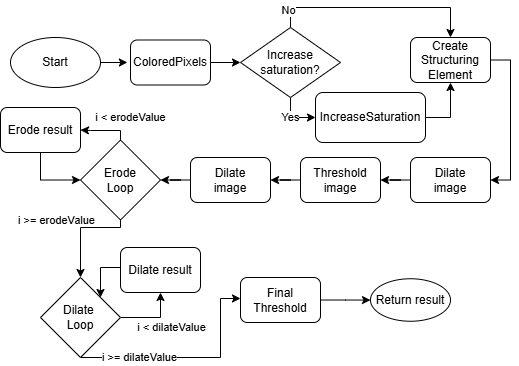
\includegraphics[width=0.9\linewidth]{img/diagram.png}
    \caption{Diagram funkcie \texttt{GetAnonymizedParts}}
    \label{fig:6.3}
\end{figure}
\subsection{Testovanie}
Vývoj prebiehal na verzovacom systéme git a je uložený na školskej inštancii gitlab \cite{lukassalak}, v repozitári je pripravená CI/CD pipeline na automatický build a automatické spustenie testov. Na obrázku \ref{fig:6.4} vidíme pokrytie testami sprostredkované frameworkom coverlet\cite{coverlet}.

\begin{figure}[H]
    \centering
    \fbox{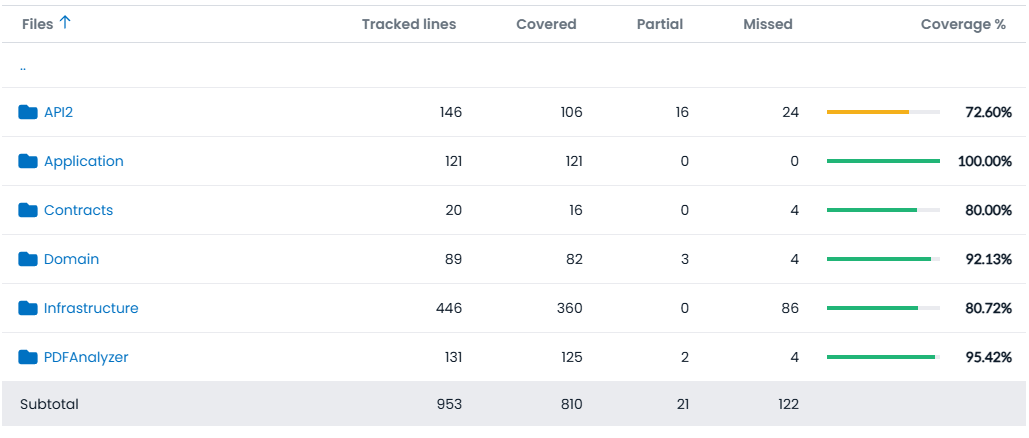
\includegraphics[width=0.7\linewidth]{img/pokrytie.png}}
    \caption{Pokrytie testov jednotlivých častí softvéru\cite{coverlet}}
    \label{fig:6.4}
\end{figure}
\end{hyphenrules}

\chapwithtoc{Záver}

In the conclusion, you should summarize what was achieved by the thesis. In a few paragraphs, try to answer the following:
\begin{itemize}
\item Was the problem stated in the introduction solved? (Ideally include a list of successfully achieved goals.)
\item What is the quality of the result? Is the problem solved for good and the mankind does not need to ever think about it again, or just partially improved upon? (Is the incompleteness caused by overwhelming problem complexity that would be out of thesis scope\todo{This is quite common.}, or any theoretical reasons, such as computational hardness?)
\item Does the result have any practical applications that improve upon something realistic?
\item Is there any good future development or research direction that could further improve the results of this thesis? (This is often summarized in a separate subsection called `Future work'.)
\end{itemize}


\ifEN
\chapwithtoc{Bibliography}
\else
\chapwithtoc{Zoznam použitej literatúry}
\fi

\printbibliography[heading=none]


\appendix
\chapter{Príloha: Implementácia riešenia}

% Use this appendix to tell the readers (specifically the reviewer) how to use your software. A very reduced example follows; expand as necessary. Description of the program usage (e.g., how to process some example data) should be included as well.

% To compile and run the software, you need dependencies XXX and YYY and a C compiler. On Debian-based Linux systems (such as Ubuntu), you may install these dependencies with APT:
% \begin{Verbatim}
% apt-get install \
%   libsuperdependency-dev \
%   libanotherdependency-dev \
%   build-essential
% \end{Verbatim}

% To unpack and compile the software, proceed as follows:
% \begin{Verbatim}
% unzip coolsoft.zip
% cd coolsoft
% ./configure
% make
% \end{Verbatim}

% The program can be used as a C++ library, the simplest use is demonstrated in \cref{lst:ex}. A demonstration program that processes demonstration data is available in directory \verb|demo/|, you can run the program on a demonstration dataset as follows:
% \begin{Verbatim}
% cd demo/
% ./bin/cool_process_data data/demo1
% \end{Verbatim}

% After the program starts, control the data avenger with standard \verb-WSAD- controls.

% \begin{listing}
% \begin{lstlisting}
% #include <CoolSoft.h>
% #include <iostream>

% int main() {
% 	int i;
% 	if(i = cool::ProcessAllData()) // returns 0 on error
% 		std::cout << i << std::endl;
% 	else
% 		std::cerr << "error!" << std::endl;
% 	return 0;
% }
% \end{lstlisting}
% \caption{Example program.}
% \label{lst:ex}
% \end{listing}


% if your attachments are complicated, describe them in a separate appendix
%\include{attachments}

%\openright
\end{document}
